\chapter{Applicazione per analisi stabilometrica}
\label{cap:applicazione_per_analisi_stabilometrica}

\section{Precedente sviluppo per Android}
Inizialmente questa tesi prevedeva lo sviluppo di un'applicazione nativa solo per piattaforma Android, per un certo periodo di tempo si è lavorato allo sviluppo di un prototipo utilizzando il linguaggio di programmazione Java per la parte sensibile di raccolta dei dati dai sensori e il linguaggio Kotlin per tutto ciò che riguarda la grafica e l'interazione con l'utente. Si è scelto di utilizzare in maggior parte Kotlin sia perché è il linguaggio ad oggi consigliato da Google per lo sviluppo Android, sia per le sue caratteristiche che riducono di molto il tempo di sviluppo e risultano in un codice più "pulito" e facile da leggere rispetto al tradizionale Java. 

Kotlin è un linguaggio di programmazione multi-paradigma basato sulla Java Virtual Machine (JVM), ciò significa che è compatibile al 100\% con Java; in particolare è orientato verso la programmazione ad oggetti (OOP) permettendo però un pieno uso dei concetti della programmazione funzionale come ad esempio le first-class functions e l'immutabilità dei dati, molto usata nelle collezioni e nelle mappe. Una delle funzionalità più notevoli di Kotlin è il {\itshape non-null by default}, ciò significa che le variabili non possono assumere valore nullo se non specificato risparmiandoci numerosi null-check ed eliminando i tanto temuti {\itshape NullPointerException}.

Arrivati ad un buon punto nello sviluppo del prototipo Android sono stati presi in considerazione diversi fattori, il più importante era la mancanza di un corrispettivo per IOS che non richiedesse lo sviluppo di un'applicazione completa, inoltre si è vista la disponibilità di più tempo per la consegna della tesi e si è deciso di scartare il prototipo e realizzarne un altro utilizzando il framework Flutter.

\section{Flutter}
Flutter è un framework open-source creato da Google per lo sviluppo di applicazioni native iOS, Android, web e desktop partendo da un'unica codebase scritta sfruttando il linguaggio di programmazione Dart.

Il componente fondamentale di un'applicazione Flutter è il {\bfseries Flutter Engine}; scritto prevalentemente in C++, è colui che gestisce il ciclo vitale della macchina virtuale Dart oltre ad interfacciarsi con gli SDK nativi delle piattaforme e a fornire il supporto per il rendering a basso livello utilizzando la libreria grafica Skia, anch'essa sviluppata da Google.
Una particolarità molto apprezzata del Flutter Engine è la possibilità di effettuare un {\itshape "hot reload"} dell'applicazione in cui le modifiche al codice sono immediatamente pubblicate senza bisogno di un riavvio completo o un cambio di stato, riducendo di molto i tempi d'attesa durante lo sviluppo.

Ciò che differenzia Flutter dagli strumenti comunemente usati per lo sviluppo mobile (Kotlin, Swift, ecc) è il paradigma reattivo (Reactive programming) il quale si basa su stream di dati e sulla propagazione dei cambiamenti.
Flutter si avvale di un approccio dichiarativo per quanto riguarda la grafica, l'idea principale è che {\bfseries la UI è una funzione dello stato}, ovvero l'interfaccia utente è ricostruita ad ogni cambiamento di stato applicando ad esso determinate funzioni definite dai Widget. 
Un Widget ha il compito di descrivere quale sarà l'aspetto della vista partendo dalla sua configurazione attuale e dallo stato; quando lo stato cambia il widget ricrea la UI con le nuove informazioni. Il Widget può essere considerato l'atomo, l'elemento più piccolo, della programmazione in Flutter; {\bfseries in Flutter tutto è un Widget}, l'applicazione è costruita componendo widget più semplici uno con l'altro ottenendo un {\itshape Widget Tree} che descrive l'intera applicazione.

\section{Prototipo dell' interfaccia utente con Figma}
Lo sviluppo di una UI può risultare particolarmente complesso, per questo motivo al posto di realizzare l'interfaccia utente direttamente in-code, sprecando tempo ed energia utile, si è deciso di realizzare un prototipo dell'aspetto grafico e delle interazioni di base fra le diverse schermate dell'applicazione.
Il mock è stato realizzato grazie al popolare strumento di design Figma.

Figma è un'applicazione di UI/UX design basata sul browser che permette di realizzare facilmente e velocemente dei prototipi di design.

Di seguito sono riportate le schermate principali e le loro funzionalità:
\begin{itemize}
  \item Home [Figura \ref{fig:home}], come dice il nome è la prima schermata che l'utente vede appena l'applicazione è caricata, essa fornisce l'accesso alla funzionalità principale: la possibilità di eseguire un test della postura. Qui l'utente può comunicare se il test che eseguirà sarà svolto ad occhi aperti oppure chiusi e, premendo il pulsante {\itshape start test} farà appunto partire la prova.

  \item Calibrazione del dispositivo [Figura \ref{fig:calibrate}], in questa schermata l'utente può eseguire la calibrazione dei sensori presenti nel suo dispositivo; questo è fatto al fine di eguagliare l'esperienza di test fra i numerosi smartphone che montano sensori di marca e modello più disparati e che possono avere degli errori nella fasatura di fabbrica.
Durante la calibrazione l'utente è esortato ad appoggiare il suo dispositivo a "faccia in su" su una superficie piana, ad esempio un tavolo, per 10 secondi. Al termine del processo vengono generati dei bias per gli assi di ogni sensore i quali saranno poi opportunamente sottratti dai dati ricavati nei test; è importante notare che una volta calcolati i bias rimangono costanti per ogni test e possono variare solo se si riesegue la calibrazione.
La prima volta che l'applicazione è avviata l'utente sarà portato ad eseguire una prima calibrazione non appena tenterà di eseguire un test, in questo modo si è certi che il dispositivo sia calibrato.

  \item Results [Figura \ref{fig:result}], qui sono mostrate all'utente tutte le informazioni ricavate da uno specifico test.
Le diverse informazioni sono racchiuse in varie carte: la prima contiene i grafici di statokinesigramma e stabilogramma, la seconda le features nel dominio del tempo, la terza le features nel dominio della frequenza, la quarta le features strutturali e l'ultima quelle giroscopiche. Qui l'utente ha anche la possibilità di esportare l'intero test in un file formato {\bfseries json} salvato nella memoria esterna (pubblica) del suo dispositivo. Si è scelto il formato json per la sua semplicità nel rappresentare i dati e per l'ottimo supporto nativo in flutter.

  \item Durante il primo avvio l'utente non è portato subito nella home, ma in una schermata d'introduzione con diverse pagine [Figura \ref{fig:onboarding}] nelle quali si da il benvenuto all'utente, si spiega lo scopo dell'applicazione e si chiedono i dati d'anamnesi; questa parte può anche essere saltata poiché le informazioni non sono obbligatorie.
\end{itemize}

\begin{figure}
  \centering
  \begin{subfigure}[b]{0.33\textwidth}
      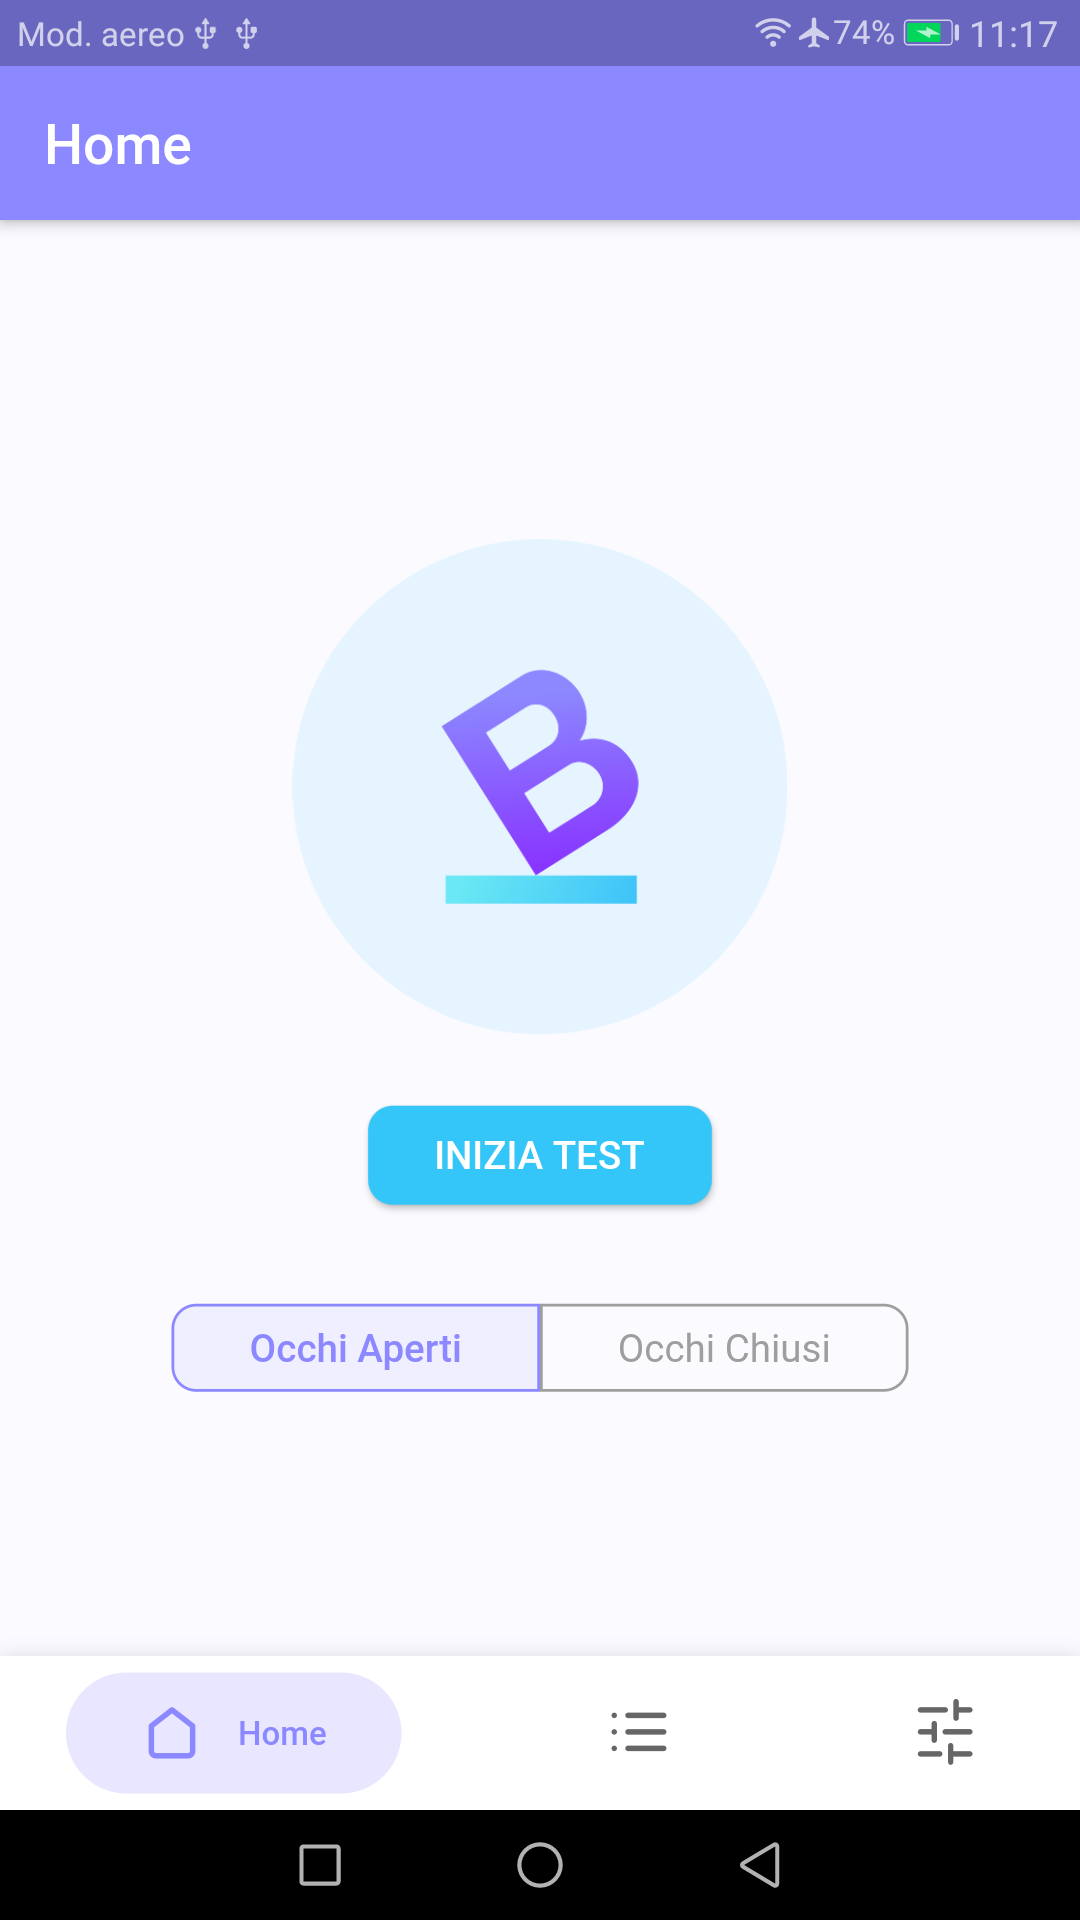
\includegraphics[width=\textwidth]{figures/screenshot/home.png}
      \caption{Pagina principale}
      \label{fig:home}
  \end{subfigure}
  \hspace{0.15\textwidth}%
  \begin{subfigure}[b]{0.33\textwidth}
      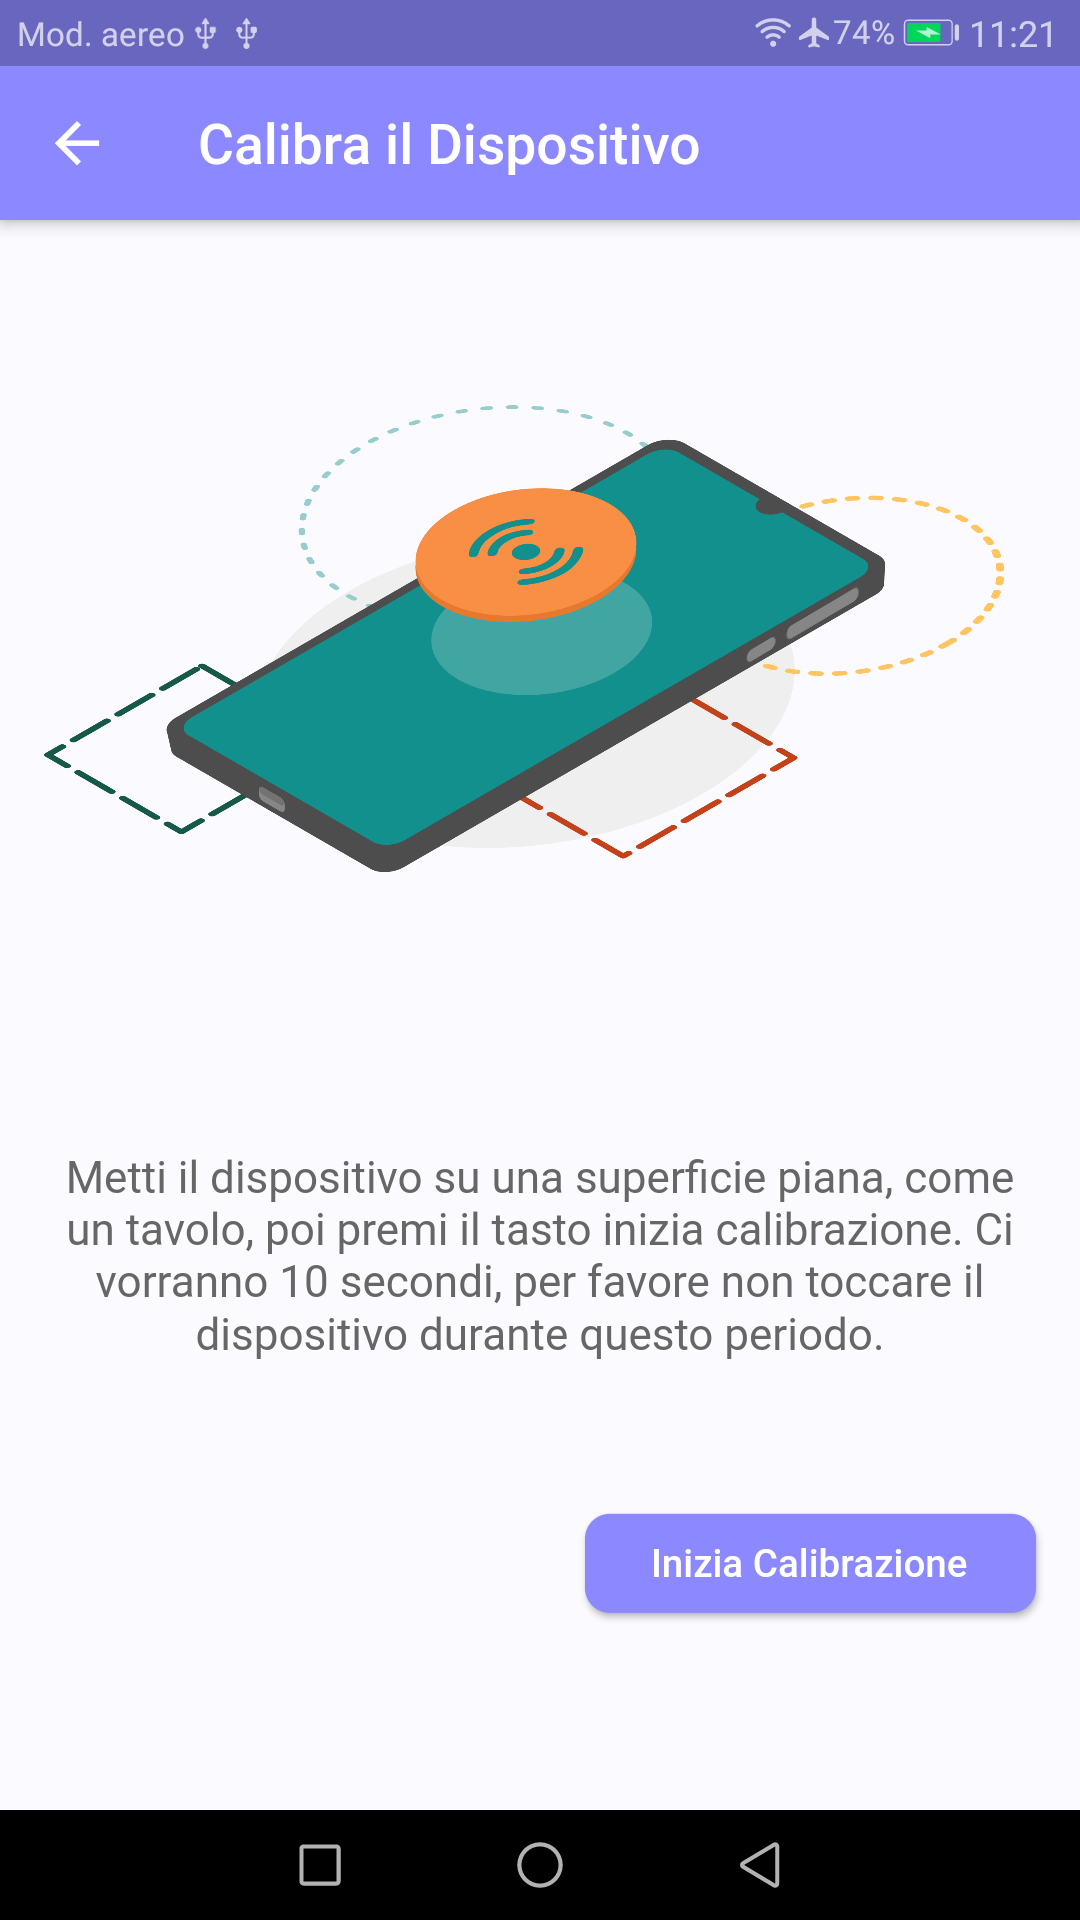
\includegraphics[width=\textwidth]{figures/screenshot/calibrate.png}
      \caption{Pagina di calibrazione del dispositivo}
      \label{fig:calibrate}
  \end{subfigure}
  \vfill
  \begin{subfigure}[b]{0.33\textwidth}
      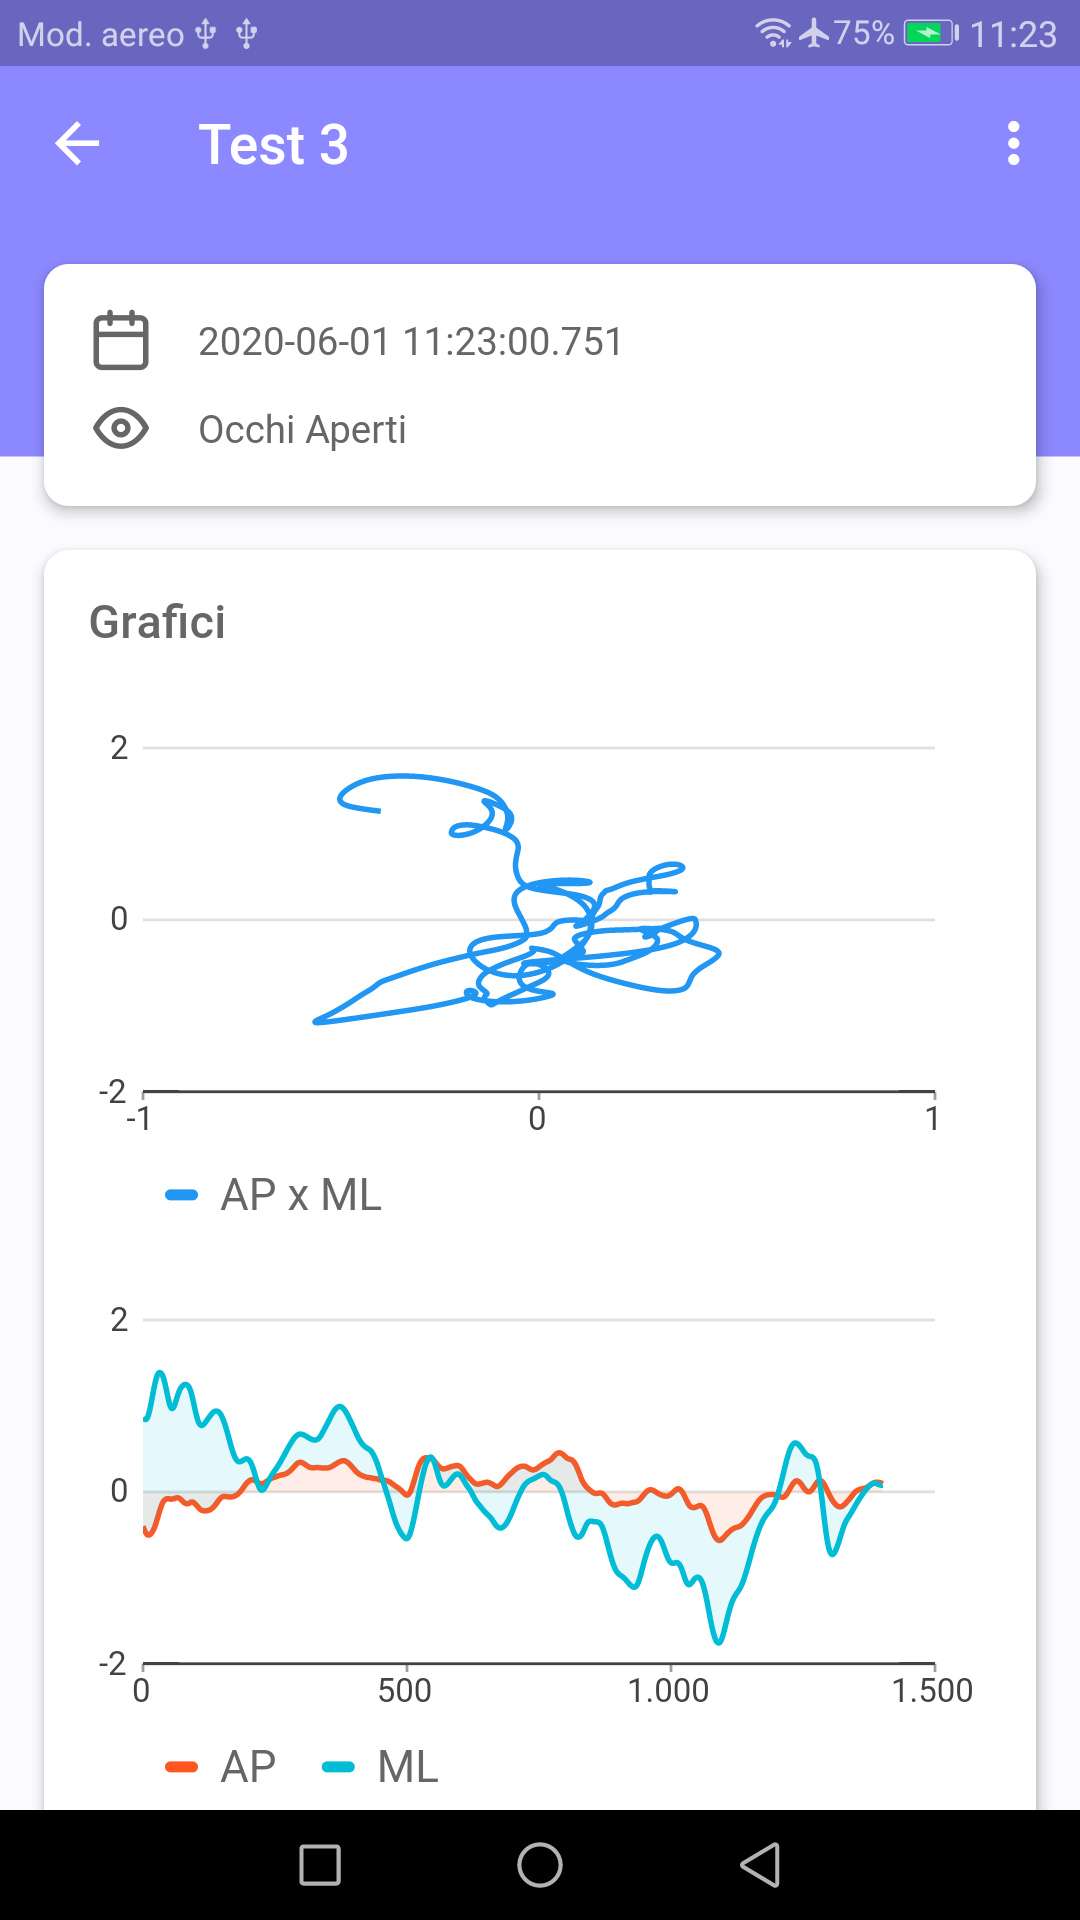
\includegraphics[width=\textwidth]{figures/screenshot/result.png}
      \caption{Pagina con i risultati di un test}
      \label{fig:result}
  \end{subfigure}
  \hspace{0.15\textwidth}%
  \begin{subfigure}[b]{0.33\textwidth}
      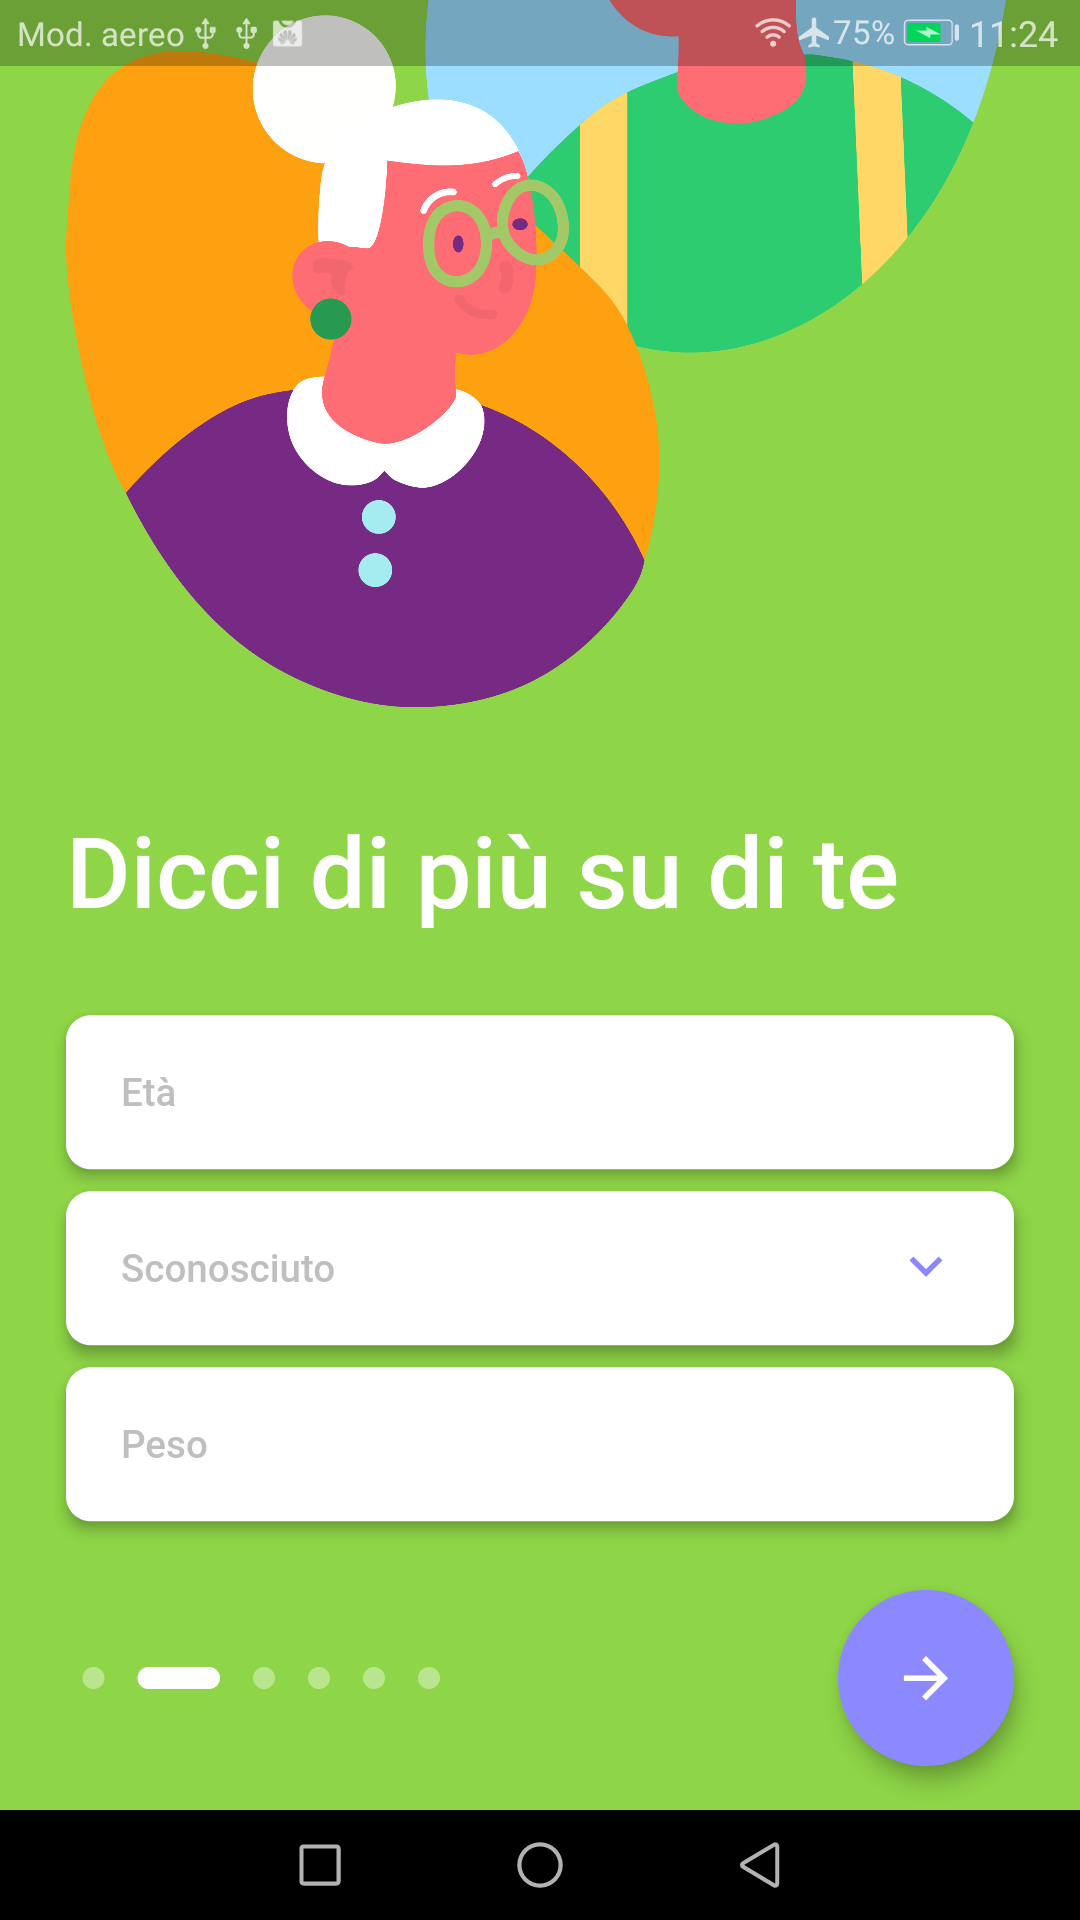
\includegraphics[width=\textwidth]{figures/screenshot/general_info.png}
      \caption{Una delle pagine in cui si chiedono i dati d'anamnesi}
      \label{fig:onboarding}
  \end{subfigure}
  \caption{Esempio di alcune delle schermate dell'applicazione}
  \label{fig:accelerometer_gyroscope}
\end{figure}

\newpage
\section{I dati d'anamnesi}
L'applicazione è progettata in modo da garantire all'utente il completo anonimato, per questa tesi si è scelto di non interfacciare l'applicazione con un database esterno, ma di salvare tutto in maniera privata all'interno del dispositivo dell'utente.

Anche se in completo anonimato all'utente vengono chieste alcune informazioni personali: la principale è la sua altezza; essa è utilizzata dall'algoritmo che estrae i COGv partendo dall'accelerometro (equazione del Capitolo \ref{cap:analisi_stabilometriche}) ed è essenziale per una corretta stima della postura. I restanti dati d'anamnesi non obbligatori sono:
\begin{itemize}
  \item l'età
  \item il genere
  \item il peso
  \item eventuali problemi posturali
  \item la presenza di problemi posturali in famiglia
  \item l'utilizzo di medicinali che possono interferire con la postura
  \item eventuali altri traumi
  \item difetti visivi
  \item difetti uditivi
\end{itemize}

Al momento all'utente è richiesta solo una piccola parte di tutti i possibili dati d'anamnesi poiché non è questo lo scopo della tesi, ma in futuro sarà possibile estenderli ed utilizzarli, assieme ai dati posturali ricavati dai vari test, per eseguire studi di correlazione.

\section{Il test della postura}
Come detto anche in precedenza lo scopo principale dell'applicazione è eseguire i test della postura, l'idea è che ogni test sia fattibile in pochi secondi e possa essere eseguito quante volte si vuole. Il test della postura si può effettuare ad occhi aperti oppure chiusi, scegliendo l'opportuna voce nella schermata home. Prima del test vero e proprio viene mostrato un contatore di 5 secondi in modo che l'utente abbia il tempo per mettersi in posizione. La postura corretta per eseguire il test è in piedi, stando più dritti possibile, guardando avanti e tenendo il dispositivo con due mani circa ad altezza ombelico.
La misurazione dei sensori vera e propria dura 32 secondi; i primi due secondi devono essere rimossi poiché possono contenere "rumore" prodotto dall'utente non ancora in posizione, questo ci lascia un campione di 30 secondi, molto simile a quello ottenuto dalle pedane stabilometriche.

\section{Plugin per la lettura dei sensori}
Un plugin in Flutter è una libreria di codice in grado di chiamare API specifiche della piattaforma, per questo esso contiene non solo codice scritto in Dart, ma anche parti di codice "nativo", scritto nel linguaggio di sviluppo della piattaforma (Kotlin/Java per Android, Swift/ObjectiveC per IOS), in questo modo è possibile ottenere più prestazioni, e utilizzare funzionalità specifiche per la piattaforma.

Per quest'applicazione in particolare, si ha il bisogno di leggere i risultati prodotti dai sensori per un periodo di tempo configurabile a priori avendo la possibilità di annullarlo prima del termine e, cosa più importante, che l'intera sequenza ottenuta abbia una frequenza di campionamento attorno a 100Hz.

Con queste specifiche in mente si è pensato di utilizzare {\bfseries sensors}\cite{sensors}, un plugin nativo di Flutter appositamente creato per ricevere tutti i dati dei sensori, purtroppo dai test effettuati al momento dello sviluppo il plugin non era in grado di produrre sequenze con sample rate maggiore di 8-10Hz, molto al disotto del target, per questo motivo si è scelto di creare da zero un plugin che risolvesse tutti i problemi.

Il plugin è sviluppato in questo modo: la classe \mintinline{dart}{SensorMonitor} è l'entry point del codice lato dart, al suo interno è presente un \mintinline{dart}{EventChannel}, un oggetto nativo di flutter con lo scopo di fare da tramite per i messaggi da e verso le piattaforme native. 
\begin{minted}{dart}
class SensorMonitor {
    static const EventChannel _defaultSensorsEventChannel = const EventChannel("uniurb.it/sensors/stream");

    /// Default constructor
    SensorMonitor([this.duration = const Duration(milliseconds: 5000)]):
    _sensorsEventChannel = _defaultSensorsEventChannel,
    _sensorsMethodChannel = _defaultSensorsMethodChannel,
    _sensorsData = [];
    
    // ...
}
\end{minted}
Quando il getter \mintinline{dart}{sensorStream} è chiamato l'EventChannel produce uno \mintinline{dart}{StreamController}. Lo StreamController ha il compito di far partire un timer per la durata settata nel costruttore, di gestire la cancellazione preventiva o al termine del countdown e di salvare in una lista i risultati ottenuti.
\begin{minted}{dart}
Stream<Duration> get sensorStream {
  _streamController ??= StreamController.broadcast(
    onListen: () {
      _sensorsData.clear();
      _sensorsStreamSubscription = _sensorsEventChannel
        .receiveBroadcastStream()
        .map((event) => eventToSensorData(event))
        .listen((event) {
          if (event != null)
            _sensorsData.add(event);
        });
      _countdownTimer = CountdownTimer(duration, Duration(milliseconds: 1000))
        ..listen((event) => _streamController.add(event.elapsed),
          onDone: () {
            // If the StreamController is not null close it
            _streamController?.close();
          }
        );
    },
    onCancel: () {
      if (_countdownTimer.isRunning)
        _countdownTimer.cancel();
      _sensorsStreamSubscription.cancel();
      _streamController = null;
    },
  );
  return _streamController?.stream;
}
\end{minted}
Il metodo \mintinline{dart}{eventToSensorData} mappa i messaggi ottenuti dalla piattaforma nativa in \mintinline{dart}{SensorData}, oggetti che rappresentano i dati di tutti i sensori.
\begin{minted}{dart}
static SensorData eventToSensorData(List event) {
  try {
    int timestamp = event[0] as int;
    int accuracy = event[1] as int;
    double accX = event[2] as double;
    double accY = event[3] as double;
    double accZ = event[4] as double;
    double gyroX = event[5] as double;
    double gyroY = event[6] as double;
    double gyroZ = event[7] as double;
    return SensorData(
      timestamp,
      accuracy,
      accX,
      accY,
      accZ,
      gyroX,
      gyroY,
      gyroZ
    );
  } catch (_) {
    return null;
  }
}
\end{minted}
Dal lato nativo, nel metodo \mintinline{kotlin}{onListen} della classe \mintinline{kotlin}{SensorMonitor} viene inizializzata una porzione di memoria condivisa, si inizia l'ascolto dei sensori ed è creata una thread pool con un singolo thread.
\begin{minted}{kotlin}
override fun onListen(arguments: Any?, events: EventChannel.EventSink?) {
  mSharedValues.reset()
  mSensorListener.startListening()
  mThreadPool = Executors.newSingleThreadExecutor()
  mThreadPool?.execute(SensorPollingRunnable(
    mUiThreadHandler,
    Runnable {
      events?.success(SensorData.mergeSensorData(
        mSharedValues.currentAccelerometerValue,
        mSharedValues.currentGyroscopeValue
      ))
    })
  )
}
\end{minted}
Il thread parallelo \mintinline{kotlin}{SensorPollingRunnable} contiene un semplice while loop nel quale esegue un \mintinline{kotlin}{Thread.sleep()} per 10 millisecondi poi prende il valore più recente di ogni sensore nella memoria condivisa e, dopo averli convertiti in una lista di numeri li invia al codice dart come massaggio attraverso l'EventChannel.

L'esempio di codice nativo viso sopra è scritto in Kotlin, non vi sono esempi da mostrare di codice per la piattaforma IOS. Lo sviluppo di codice Swift/ObjectiveC è possible da qualsiasi ambiente di lavoro in maniera gratuita, però per poter testare il corretto funzionamento è richiesto un dispositivo IOS reale oppure un emulatore il quale è disponibile solo per dispositivi apple, per questo motivo è stato lasciato come sviluppo futuro.

\section{Il calcolo delle features e il Flutter Isolate}

L'algoritmo per il calcolo delle features è composto da 3 passaggi:
\begin{enumerate}
  \item il {\itshape raw} input è convertito in liste per gli assi di accelerometro e giroscopio
  \item i valori di COGvAP e COGvML sono calcolati partendo dai dati dell'accelerometro, internamente tutti i dati sono rappresentati sotto forma di matrici per poi estrarli in due liste al termine 
  \item le features sono calcolate utilizzando i valori di COGv e del giroscopio
\end{enumerate}

L'intero algoritmo è inserito all'interno della funzione \mintinline{dart}{compute} nativa di Flutter la quale consente di eseguire l'intero codice dentro ad un Flutter Isolate. Dart è un linguaggio single thread, ciò significa che le istruzioni sono eseguite una alla volta; per ottenere asincronia si utilizza un Event Loop. Nel caso occorra eseguire operazioni molto lente o pesanti il Flutter Isolate consente di ottenere un diverso Event Loop nel quale eseguire il codice di fatto in maniera parallela al precedente. Gli Isolate, come dice il nome, sono spazi di memoria isolati, con i quali è possibile scambiare dati solo tramite messaggi.

\section{Contributi all'Open Source}

{\bfseries Pub} è il package manager del linguaggio Dart, contenente librerie e pacchetti riusabili per Dart e Flutter; qui chiunque può sviluppare e pubblicare il proprio pacchetto o utilizzare quelli degli altri nei suoi progetti come dipendenze. Un pacchetto solitamente è un insieme di file e classi che risolvono uno specifico problema o aggiungono una determinata funzionalità.

Durante lo sviluppo dell'applicazione si è notato varie volte che alcune funzionalità potevano essere estratte come dipendenze esterne, così si è colta l'occasione per creare diversi pacchetti e pubblicarli su pub.dev 
\begin{itemize}
  \item custom\_dropdown\cite{cudropdown} fornisce una semplice dropdown con uno stile diverso da quello di default
  \item iirjdart\cite{iirjdart} è il porting in dart della libreria iirj scritta in java. Questo pacchetto fornisce le funzionalità di filtro passa alto, passa basso, passa banda ed elimina banda di tipo Butterworth, Bessel e Chebychev di tipo 1 e 2.
  \item powerdart\cite{powerdart} è un pacchetto dart per stimare la densità spettrale di potenza(PSD) ed analizzarne i risultati. Al suo interno sono presenti metodi per il calcolo della PSD e per il calcolo integrale utilizzando il metodo dei trapezi.
  \item about\_dependencies\cite{abtdependencies} ha l'obbiettivo di generare un file dart con all'interno la lista di tutte le dipendenze utilizzate nel progetto e le loro informazioni base (versione, descrizione). Questo pacchetto è particolare perché, a differenza delle altre dipendenze che vengono utilizzate dall'applicazione, questa è impiegata solo durante la fase di sviluppo ed è il file generato a far parte dell'applicazione finale.
\end{itemize}